%%%%%% CMB-S4 Neutrinos Chapter  %%%%%%%%%%%%%%%%
 
\chapter{Neutrinos and Light Species from the Cosmic Microwave Background}
%\renewcommand*\thesection{\arabic{section}}


\def\beq{\begin{equation}}
\def\eeq{\end{equation}}

\def\bea{\begin{eqnarray}}
\def\eea{\end{eqnarray}}

\def\Neff{N_{\rm eff}}
\def\Nf{N_{\rm eff}}
\def\gs{g_{\star}}
\def\Mpl{M_{\rm pl}}
\newcommand{\nucl}[3]{ \ensuremath{ \phantom{\ensuremath{^{#1}_{#2}}} \llap{\ensuremath{^{#1}}} \llap{\ensuremath{_{\rule{0pt}{.75em}#2}}} \mbox{#3} } }


\def\gtrsim{\raise-.75ex\hbox{$\buildrel>\over\sim$}}
\def\lsim{\raise-.75ex\hbox{$\buildrel<\over\sim$}}
%%%%%%%%%%%%%%%%%%%%%%%%%%%%%%%%%%%%%%%%%%%%%%%%%%%%%%%%%%%
%%%%%%%%%%%%%%%%%%%%%%%%%%%%%%%%%%%%%%%%%%%%%%%%%%%%%%%%%%%
%%%%%%%%%%%%%%%%%%%%%%%%%%%%%%%%%%%%%%%%%%%%%%%%%%%%%%%%%%%
%%%%%%%%%%%%%%%%%%%%%%%%%%%%%%%%%%%%%%%%%%%%%%%%%%%%%%%%%%%

\begin{center}
{\small \it (send feedback on this chapter to \href{mailto:s4_neutrinos@cosmo.uchicago.edu}{s4\_neutrinos@cosmo.uchicago.edu})}
\end{center}

\section{Introduction}



Direct interactions between neutrinos and observable matter effectively ceased about one second after the end of inflation.  Nevertheless, the total energy density carried by neutrinos was comparable to other components through recent cosmological times.  As a result, the gravitational effect of the neutrinos is detectable both at the time of recombination and in the growth of structure at later times~\cite{Abazajian:2013oma}, leaving imprints in the temperature and polarization spectrum as well as in CMB lensing.

CMB-S4 can improve our understanding of neutrino physics in regimes of interest for both cosmology and particle physics.  Arguably the most important parameters of interest will be the sum of the neutrino masses ($\sum m_\nu$) and the effective number of neutrino species ($\Neff$).  These two parameters have natural targets that are within reach of a CMB-S4 experiment:
\begin{itemize}
\item $ \sum m_\nu \gtrsim \, 58$ meV is the lower bound guaranteed by observations of solar and atmospheric neutrino oscillations.  A CMB experiment with $\sigma(\sum m_\nu) < 20$ meV would be guaranteed a detection of a least 3$\sigma$.  At this level, one can detect the overall scale of the neutrino masses even for a normal ordered hierarchy.
\item $\Delta \Neff \geq  0.027, \, 0.047$, and $0.054$ are predicted for models containing additional light particles of spin $0$, $1/2$ and $1$ that were in thermal equilibrium with the particles of the Standard Model.  A CMB experiment reaching $\sigma(\Neff) \lesssim 0.01$ would be sensitive to all models in this very broad class of extensions of the Standard Model, which includes a wide range of models predicting axions and axion-like particles.  At lower sensitivity ($\sigma(\Neff) \lesssim 0.03$), we can test the full range of models containing light fermions and vectors, including gravitinos and dark photons that freeze-out before the QCD phase transition.  
\end{itemize}
Current CMB data already provides a robust detection of the cosmic neutrino background at $\sim10 \sigma$.  A CMB-S4 experiment will provide an order of magnitude improvement in sensitivity that opens a new window back to the time of neutrino decoupling and beyond.

Section 2 will review the motivation for studying neutrino masses with cosmological probes, and specifically with the CMB.  We will explain why cosmology is sensitive to $\sum m_\nu$ via different probes and how it is complementary to the laboratory-based experimental neutrino effort.  Section 3 will review the physics of $\Neff$ and its role as probe of the C$\nu$B and as sensitive tool for beyond the Standard Model physics.  We will emphasize the unique impact $\Neff$ has on the CMB that makes it distinguishable from other extensions of $\Lambda$CDM.  In Section 4, we will discuss the implications for a variety of well motivated models, including sterile neutrinos and axions.  In Section 5, we will discuss the relation between CMB and BBN based constraints.  

\section{Neutrino Mass}

\subsection{Theory Review}

Cosmic background neutrinos are nearly as abundant in the universe as CMB photons. In the standard cosmological model, neutrinos ceased to scatter with other particles at temperatures $\sim 1 \, {\rm MeV}$. The relic neutrinos were relativistic at decoupling, but as the universe expanded and cooled the neutrino momenta redshifted as $p_\nu\propto 1/a$ and eventually the energy of most relic neutrinos came to be dominated by their rest mass, rather than their momentum. The energy density in nonrelativistic neutrinos therefore contributes to the matter budget of the universe today. The neutrinos, however, were relativistic for much of the history of the Universe so their gravitational clustering is qualitatively different from that of cold dark matter (CDM) particles. This difference can be used to distinguish the neutrino and cold dark matter contributions to the matter density \cite{Hu:1997mj, Lesgourgues:2006nd, Abazajian:2011dt}.  In this section, we review how neutrino mass affects the evolution of the neutrino energy density and the gravitational clustering of matter in the universe. 
 
As discussed more detail in the $\Neff$ section, cosmic background neutrinos have been detected indirectly through their contribution to the energy density in radiation in the early universe. The current CMB constraints from $\Neff$ are in excellent agreement with the Standard Model expectation of three species of neutrinos and anti-neutrinos each described by a relativistic thermal Fermi-Dirac distribution \cite{Ade:2015xua}. The distribution function for each species of neutrinos and anti-neutrinos is given by
\beq
f_\nu(p) = \frac{1}{e^{a p/(k_BT_{\nu 0})} +1} \ ,
\eeq
where $T_{\nu 0} \approx 1.95K$ or $k_B T_{\nu 0} \approx 1.68 \times 10^{-4}\,{\rm eV}$ is the temperature today. Note that the spectral shape of the neutrino phase space distribution is preserved with the expansion of the universe so relic neutrinos have retained the relativistic Fermi-Dirac momentum distribution inherited from decoupling even as the individual neutrinos became non-relativistic. 

The neutrino energy density is given by
\beq
\rho_\nu = \sum_i \int\frac{d^3 {\bf p}}{(2\pi \hbar)^3} \frac{\sqrt{p^2 + m_{\nu i}^2}}{e^{ap/(k_BT_{\nu 0})} +1}
\eeq
where $m_{\nu i}$ are the three neutrino mass eigenstates.  For $T_{\nu}/a \gg m_{\nu i}$ the neutrino energies are dominated by their momenta and the total energy density behaves like radiation
\bea
\rho_{\nu}\Bigg|_{{\rm {\tiny early}}}  &\approx& \frac{7 \pi^2}{40}\frac{(k_B T_{\nu 0})^4}{\hbar^3 c^3}\frac{1}{a^4} \\
& \propto& a^{-4} \nonumber
\eea
While for $T_{\nu 0}/a \ll m_{\nu i}$ the energy density behaves like matter
\bea
\label{eq:rhonumassive}
\rho_{\nu} \Bigg|_{{\rm {\tiny late}}}  &\approx& \sum_i m_{\nu i} \bar{n}_\nu \\
&\propto& a^{-3} \nonumber
\eea
where $\bar{n}_\nu$ is the number of neutrinos and antineutrinos in each mass eigenstate
\beq
\bar{n}_\nu =\int\frac{d^3 {\bf p}}{(2\pi \hbar)^3} \frac{2}{e^{ap/(k_BT_{\nu 0})} +1} \approx \frac{113}{a^3}\,{\rm cm}^{-3}\,.
%&=&  \frac{6 \zeta(3)}{4\pi^2} \left(\frac{k_B T_\nu}{\hbar c}\right)^3\frac{1}{a^3}\\
\eeq

For a neutrino of mass $m_{\nu i}$ the transition between these two regimes ($T_\nu(a) \sim m_{\nu i}$) occurs at redshift $z_{\rm nr} \sim 300 (m_{\nu i}/0.05 {\rm eV})$. Using Eq.~(\ref{eq:rhonumassive}) the fractional energy density in neutrinos today can be written as
\beq
\Omega_\nu h^2 \approx \frac{\sum_i m_{\nu i}}{93\,{\rm eV}}\,.
\eeq
The individual masses of the neutrino states are unknown but neutrino oscillation data specifies the square of two mass splittings $\Delta m_{12}^2 = 7.54 \times 10^{-5}$~eV, $|\Delta m_{13}^2|\approx 2.4 \times 10^{-3}$~eV \cite{Agashe:2014kda}. These mass splittings, in combination with the neutrino number density, give a lower limit on the contribution of neutrinos to the cosmic energy budget
\beq
\Omega_\nu h^2 \,  \gtrsim \, 0.0006\,.
\eeq
At $z \ll z_{\rm nr}$ the matter density of the universe, which enters into the Hubble equation, is the sum of the CDM, baryon, and massive neutrino energy densities $\Omega_m = \Omega_c + \Omega_b + \Omega_\nu$. Whereas, at $z\gg z_{\rm nr}$ the matter density is solely made up of the baryon and CDM parts while neutrinos contribute to the radiation density. 

Neutrinos do not participate in gravitational collapse until late times when they have become nonrelativistic. Prior to this transition, the neutrinos {\em free-stream} out of gravitational wells, leaving the CDM and baryons behind  \cite{Bond:1983hb, Ma:1996za, Hu:1997vi, Hu:1997mj}. Primordial fluctuations in the neutrino density are therefore damped away on scales smaller than the horizon at $z_{\rm nr}$. In comoving units, this scale corresponds to a wave number
\beq
k_{\rm nr} \equiv a_{\rm nr} H(a_{\rm nr})/c \approx 0.003 \left(\frac{\Omega_m}{0.3}\frac{m_{\nu}}{0.05\, {\rm eV}}\right)^{1/2} h/{\rm Mpc}\,.
\eeq
Once the neutrinos are non-relativistic, their finite velocity dispersion still prevents them from clustering on scales smaller than the typical distance a neutrino travels in a Hubble time, $v_\nu /H(a)$ where $v_\nu \approx 3.15 T_{\nu 0}/(a m_\nu)$ the mean neutrino velocity. In analogy with the Jeans criterion for gravitational collapse, the neutrino free-streaming scale is defined by \cite{Bond:1983hb, Lesgourgues:2006nd}
\beq
k_{\rm fs}(a) \equiv \sqrt{\frac{3}{2}}\frac{aH(a)}{v_\nu(a)} \approx 0.04\, a^2 \sqrt{\Omega_m a^{-3} + \Omega_\Lambda}\left(\frac{m_\nu}{0.05 {\rm eV}}\right) h/{\rm Mpc}
\eeq
in comoving coordinates. 

On scales larger than $k_{\rm nr}$ (adiabatic) perturbations in the density of neutrinos, baryons, and CDM are coherent and can be described by a single perturbation to the total matter density $\delta_m= \delta \rho_m/\rho_m$. On smaller scales where the neutrino perturbations have decayed, only the perturbations to the CDM and baryons remain so that $\delta_{m} = \delta_{cb}\, (\Omega_{c} + \Omega_b)/\Omega_m $. The remaining CDM and baryon perturbations also grow more slowly because the neutrino energy density contributes to the expansion rate, but not to the source potentials. These two effects cause a suppression in the amplitude and the growth rate of matter perturbations wavenumbers $k > k_{\rm fs}$ relative to a universe with massless neutrinos (and also relative to density perturbations with $k<k_{\rm nr}$). The net change in the amplitude of perturbations with $k > k_{\rm nr}$ primarily depends on the fractional energy density in massive neutrinos (keeping $\Omega_c+\Omega_b$ fixed) but retains a small sensitivity to the individual neutrino masses through a dependence on $a_{\rm nr}$. 

An estimate of the effect of massive neutrinos on the growth of structure can be made by studying the evolution of matter perturbations in the two regimes $k\ll k_{\rm fs}$ and $k\gg k_{\rm fs}$.  In the synchronous gauge, linear perturbations to the matter density with wavenumbers $k \ll k_{\rm fs}$ evolve as
\beq
\label{eq:ddotdeltalarge}
\ddot{\delta}_m + 2 H(a) \dot\delta_m - \frac{3}{2}\Omega_mH_0^2 a^{-3}\delta_m = 0\quad {\rm for }\quad k \ll k_{\rm nr}
\eeq
which has solutions $\delta_m \propto a, \, a^{-\frac{3}{2}}$ during the matter dominated era. %On these scales, the evolution of matter perturbations just depends on $\Omega_m$, not on the fractional energy density in massive neutrinos. 

On scales where the neutrino perturbations have decayed, perturbations to matter density are just in the CDM and baryon components 
\beq
\delta_m(k\gg k_{\rm fs})\approx  (\delta\rho_c + \delta\rho_b)/\rho_m = (1-f_\nu)\delta_{cb}
\eeq 
where $f_\nu = \Omega_\nu/\Omega_m$ and $\delta_{cb} = (\delta\rho_c + \delta\rho_b)/(\rho_c + \rho_b)$, but the neutrino energy density still contributes to the Hubble friction. In this limit, linear perturbations to the  CDM and baryon density evolve as
\beq
\label{eq:ddotdeltasmall}
\ddot{\delta}_{m} + 2 H(a)\dot{\delta}_{m} - \frac{3}{2}\Omega_{cb}H_0^2 a^{-3} \delta_{m} =0\quad {\rm for}\quad  k \gg k_{\rm fs} 
\eeq
where $\Omega_{cb} = \Omega_c + \Omega_b$ and $\Omega_{cb} < \Omega_m$ for a cosmology with massive neutrinos. Equation (\ref{eq:ddotdeltasmall}) has the approximate solutions during the matter dominated era of $\delta_{cb} \propto a^{1-\frac{3}{5}f_\nu}, a^{-\frac{3}{2} + \frac{3}{5}f_\nu}$ for $f_\nu  \ll 1$. \

The matter dominated solutions give a simple estimate of the net effects of massive neutrinos on the amplitude of matter perturbations. For fixed $\Omega_c h^2$, the evolution of perturbations in a cosmology with $f_\nu \neq 0$ is the same as a cosmology with $f_\nu =0$. After $a_{\rm nr}$, the perturbations with $k\gg k_{\rm fs}$ grow more slowly (according to Eq.~(\ref{eq:ddotdeltasmall}), the growing mode solution grows as  $\propto a^{1-\frac{3}{5}f_\nu}$) than those with $k\ll k_{\rm fs}$ (according to Eq.~(\ref{eq:ddotdeltalarge}), $\propto a$).  At scale-factor $a$ during the matter dominated era, the total difference in growth or perturbations with $k\gg k_{\rm fs}$ is roughly
\beq
\frac{\delta_{cb}(k \gg k_{\rm fs}, a | f_\nu)}{\delta_{cb}(k \gg k_{\rm fs}, a | f_\nu=0)} \sim \left(\frac{a}{a_{\rm nr}}\right)^{-\frac{3}{5}f_\nu}\,.
\eeq
The resulting difference in the amplitude of the matter power spectra is then 
\beq
\frac{P_{mm}(k \gg k_{\rm fs}, a  |f_\nu)}{P_{mm}(k \gg k_{\rm fs}, a |f_\nu =0)}\sim (1-2f_\nu)\frac{P_{cc}(k \gg k_{\rm fs} , a |f_\nu)}{P_{cc}(k \gg k_{\rm fs}, a |f_\nu =0)}\sim \left(1-2f_\nu -\frac{6}{5}f_\nu\ln\left(a/a_{\rm nr}\right)\right)\,.
\eeq
On the other hand, the evolution of the large scale modes is identical,
\beq
\frac{P_{mm}(k \ll k_{\rm fs}, a  |f_\nu)}{P_{mm}(k \ll k_{\rm fs}, a |f_\nu =0)}=1\,.
\eeq
The above expression overestimates the effect of neutrino mass by assuming the transition from relativistic to non-relativistic is instantaneous. It also ignores the effects of the cosmological constant at late times. Using the true evolution of $\delta_{cb}$ through $a_{\rm nr}$ and allowing for the cosmological constant gives 
\beq
\frac{P_{mm}(k \gg k_{\rm fs} |f_\nu)}{P_{mm}(k \gg k_{\rm fs} |f_\nu =0)} \approx 1- 6 f_\nu
\eeq
at $a=1$. Note that this expression assumes fixed $\Omega_ch^2$, $\Omega_bh^2$ so that matter-radiation equality is not changed by neutrino mass and that and $\Omega_\Lambda = 1-\Omega_m$ is fixed by adjusting $h$ so that the onset of cosmological constant domination is also unchanged. Alternatively, assuming fixed $\Omega_m$ and decreasing $\Omega_{cb}$ to account for $\Omega_\nu$ makes matter-radiation equality, which occurs while the neutrinos are relativistic, slightly later so that the suppression is increased to
\beq
\frac{P_{mm}(k \gg k_{\rm fs} |f_\nu)}{P_{mm}(k \gg k_{\rm fs} |f_\nu =0)} \approx (1-8f_\nu)\,.
\eeq


\subsection{CMB Lensing}

Likely the cleanest probe of the neutrino mass in the CMB is through gravitational lensing~\cite{Kaplinghat:2003bh}, which directly measures the matter distribution along the line of sight.  To be concrete, in the Limber approximation, the lensing power spectrum is given by
\bea
C_\ell^{\phi \phi} &=& \frac{8\pi^2}{\ell^2} \int^{\chi_\star}_0 \chi d\chi P_\Psi(\ell /\chi ; \eta_0 - \chi)  \frac{(\chi_\star -\chi)^2}{\chi_\star \chi} \\
P_\Psi (k;\eta)&=& \frac{9 \Omega_m^2 (\eta) H^4(\eta)}{8 \pi^2} \frac{P_{mm}(k;\eta)}{k}
\eea
where $\chi$ ($\chi_\star$) is the co-moving distance (to the last scattering surface) and $\eta$ ($\eta_0$) is conformal time (today).   More details regarding CMB lensing, including current and future measurements, will be discussed in Chapter **.

For the purposes of the neutrino mass measurement, the advantage of lensing over other probes is that it is largely free of astrophysical uncertainties.  As we see from the lensing power spectrum, we are directly sensitive to the matter power spectrum (rather than a biased tracer) and the relevant scales are in the linear regime where modeling should be reliable.

The primary challenges for the lensing measurement are degeneracies with other cosmological parameters.  The two primary degeneracies in $\Lambda$CDM are
\begin{itemize}
\item Optical depth, $\tau$: The suppression of small scale power at low redshift requires a reliable measurement of the amplitude of the power spectrum at high redshift.  In principle, this is measured by the primary CMB anisotropies, but the overall normalization is degenerate with $\tau$ for $\ell \gtrsim 20$.  A precise measurement of $\tau$ is therefore crucial to calibrate the suppression at low redshifts.  Such a measurement will likely come from $\ell \lesssim 20$ polarization data from CMB-S4 and/or other CMB experiments.  It should be emphasized that Stage IV sensitivity is not needed for the measurement of $\tau$ and such a measurement could be performed by Planck or a Stage III experiment.


\item $\Omega_m$ : The amount of lensing is controlled by the total amount of matter.  Therefore, we can compensate for a suppression from neutrinos by increasing the matter power spectrum.  This degeneracy will be broken by DESI BAO measurements of the expansion history.
\end{itemize}
In addition to degeneracies in $\Lambda$CDM there can be degeneracies with possible extensions.  Most notably:
\begin{itemize}
\item $\Neff$: The density of neutrinos after they become non-relativistic is given by $\rho_\nu \simeq m_\nu n_\nu$ where $n_\nu$ is the number density.  Therefore, we only measure the mass if we know the number density to sufficient accuracy.  Fortunately, as we will discuss in the next section, measurements of the neutrino energy density from the primary CMB will be sufficiently accurate as to make this degeneracy insignificant under plausible assumptions.
\end{itemize}
In principle, measurement of the free streaming scale directly in the matter power spectrum would separate the neutrino mass from most other physical quantities.  Unfortunately, given current limits on the neutrino mass, the change to the shape of the lensing potential power spectrum is not expected to drive future constraints.  

{\it Status of current observations} -- Planck has provided a strong constraint of $\sum m_\nu < 0.194$ eV when combining both temperature and polarization data with the CMB lensing power spectrum and external data.  A weaker constraint of $\sum m_\nu < 0.492$ eV can be derived using only the temperature and polarization data.  This constraint arises through the effect of massive neutrinos on the primordial TT and EE power spectra.  For sufficiently large masses, the neutrinos do not behave as radiation around the time of recombination which impacts the damping tail and locations of the acoustic peaks.  Improvements in the limits on the sum of the neutrino masses will be driven primarily by lensing given that current limits imply that the neutrinos are effectively massless from the point of view of the primary CMB anisotropies.  External data (BAO) will continue to be important in breaking the degeneracy with $\Omega_m$.  

\subsection{Other Cosmological Probes}

\subsection{SZ Cluster Abundance}
Galaxy clusters form from rare high peaks in the matter density field. A cluster of mass $M$ forms from a region of size $R\sim \left(M/(4/3\pi \bar\rho_m)\right)^{1/3}$, which is smaller than the neutrino free streaming scale for even the most massive galaxy clusters so long as $m_{\nu i} \lsim 0.1$eV. The neutrino free-streaming therefore slows the growth of structure on cluster scales, suppressing the abundance of galaxy clusters. 

The abundance of clusters with mass $M$ can expressed by (e.g. \cite{Tinker:2008ff, 2011ApJ...732..122B}), 
\beq
\frac{dn}{dM}(M,z) = \frac{\rho}{M}\frac{d\ln \sigma^{-1}}{dM} f(\sigma, z)
\eeq
where $\sigma = \sigma(M,z)$ is the variance of linear perturbations in CDM and baryons on mass scale $M$ given by
\beq
\label{eq:sigmaM}
\sigma^2(M, z) = \int \frac{dk}{k} \frac{4\pi}{(2\pi)^3} P_{cb}(k, z) |W(kR)|^2
\eeq
where $R = (3M/(4\pi \rho_{cb}))^{1/3}$, $P_{cb}(k)$ is the power spectrum of CDM and baryons, and $W(kR) = 3(\sin(kR)/(kR)^3 - \cos(kR)/(kR)^2)$ is a top-hat window function \cite{Costanzi:2013bha, LoVerde:2014rxa}. The cluster abundance is therefore extremely sensitive to $M_\nu$ via the suppression in the matter power spectrum discussed in the previous section. Current constraints from current constraints on neutrino mass from cluster abundance, in combination with the primary CMB and BAO, are $M_\nu \lsim 0.2 -0.3$eV at $95\%$ confidence \cite{Hasselfield:2013wf,Mantz:2014paa, Ade:2015fva,deHaan:2016qvy}. 

Galaxy clusters can be identified from CMB data via the thermal Sunyaev-Zel'Dovich (tSZ) effect, the frequency shift of CMB photons that have scattered off of electrons in the hot, intra-cluster gas \cite{sunyaev72}.  The size of the SZ signal does not provide a direct measurement of the mass of the cluster but instead is directly sensitive to the free electron density in the cluster.  As a result, determining the mass function requires calibration of the mass-signal relation.  CMB S4 is projected to detect a nearly mass-limited sample of $\mathcal{O}(100,000)$ galaxy clusters that can be used to test the neutrino mass scale. 

\subsection{CMB in Combination with Other Datasets}

There are a number synergistic opportunities between CMB S4 and external cosmological datasets. The CMB lensing convergence map can be cross-correlated with external galaxy surveys to tighten constraints on neutrino mass (e.g. \cite{Takeuchi:2013gpa, Pearson:2013iha}) or CMB can be cross-correlated with galaxy survey data to constrain neutrino mass via the mean pair-wise momentum of galaxy clusters  \cite{Mueller:2014dba}. Additionally, CMB S-4 data indirectly aid measurements of neutrino mass from galaxy surveys because the CMB data can be used to calibrate systematics in weak lensing shear data \cite{Das:2013aia}. 


\subsubsection{Relation to Other Surveys}

\subsection{Forecasts}

\begin{table}[t!]
\begin{center}
\begin{tabular}{l ccc cc} 
 \toprule
    				    			& $1'$  		& $2'$  		& $3'$  		& $\ell_{\rm max} = 3000$	& $\ell_{\rm max} = 4000$ \\ [0.5ex]
 \midrule
   $\sigma(\Neff)$ & -- 		& -- 		& --		& -- 	  	  	& -- 		  \\
    \bottomrule
\end{tabular}
\caption{Forecasts for varying beam size and maximum multipole assuming...}
\label{tab:beam}
\end{center}
\end{table}


\subsection{Relation to Lab Experiments}\label{sec:lab}

One of the more interesting connections between cosmological measurements of neutrino mass and terrestrial experiments is the complementarity between cosmological neutrino mass measurements and the search for neutrinoless double beta decay (NLDBD). NLDBD is a hypothetical decay mode of certain nuclei where two neutrons convert to two protons and two electrons with no emission of neutrinos. The observation of NLDBD would be transformational demonstrating that neutrinos are Majorana particles and revealing a new lepton-number-violating mechanism for mass generation. This new physics could potentially explain both the smallness of neutrino masses and matter-antimatter asymmetry in the universe.

Initial results from the current generation of NLDBD searches limit the NLDBD half life, $T^{0\nu}_{1/2}$, to be larger than  $\sim2\times10^{25}$~years~\cite{Agostini:2013mzu,Auger:2012ar,Artusa:2014lgv}.%\cite{Gerda, Exo, Cuore}.
 The full sensitivity of these experiments is expected to be in the range of $10^{25}-10^{26}$~years~\cite{NSAC}. Planning and technology development is already underway for next generation ``ton-scale'' NLDBD searches which would achieve sensitivities of $10^{27}-10^{28}$~years~\cite{NSAC}.

We can illustrate the connection between NLDBD searches to cosmological determinations of neutrino mass by examining the simplest case where NLDBD is mediated by exchange of light Majorana neutrinos. Within the context of this mechanism, we can define an ``effective neutrino mass,'' $m_{\beta\beta}$, given by 

\beq
m_{\beta\beta}^{2} = ( \sum_i U_{ei}^{2}m_{\nu i} )^{2}
\label{eq:mbb}
\eeq
where $m_{\nu i}$ are the light neutrino masses and $U_{ei}$ is the usual PMNS mixing matrix only including two unknown Majorana phases. The NLDBD half-life is then given by 

\beq
(T^{0\nu}_{1/2})^{-1} = G^{0\nu}\cdot (M^{0\nu} )^{2}\cdot m_{\beta\beta}^2,
\eeq

where $G^{0\nu}$ is a phase space integral and $M^{0\nu}$ is the nuclear matrix element. In this simple scenario, the signal from NLDBD experiments can be directly related to other measures of neutrino mass. Figure~\ref{fig:NLDBD} illustrates this relationship between the effective neutrino mass and the lightest neutrino mass including limits and sensitivities of current and next generation NLDBD searches.

\begin{figure}[h!]
\centering 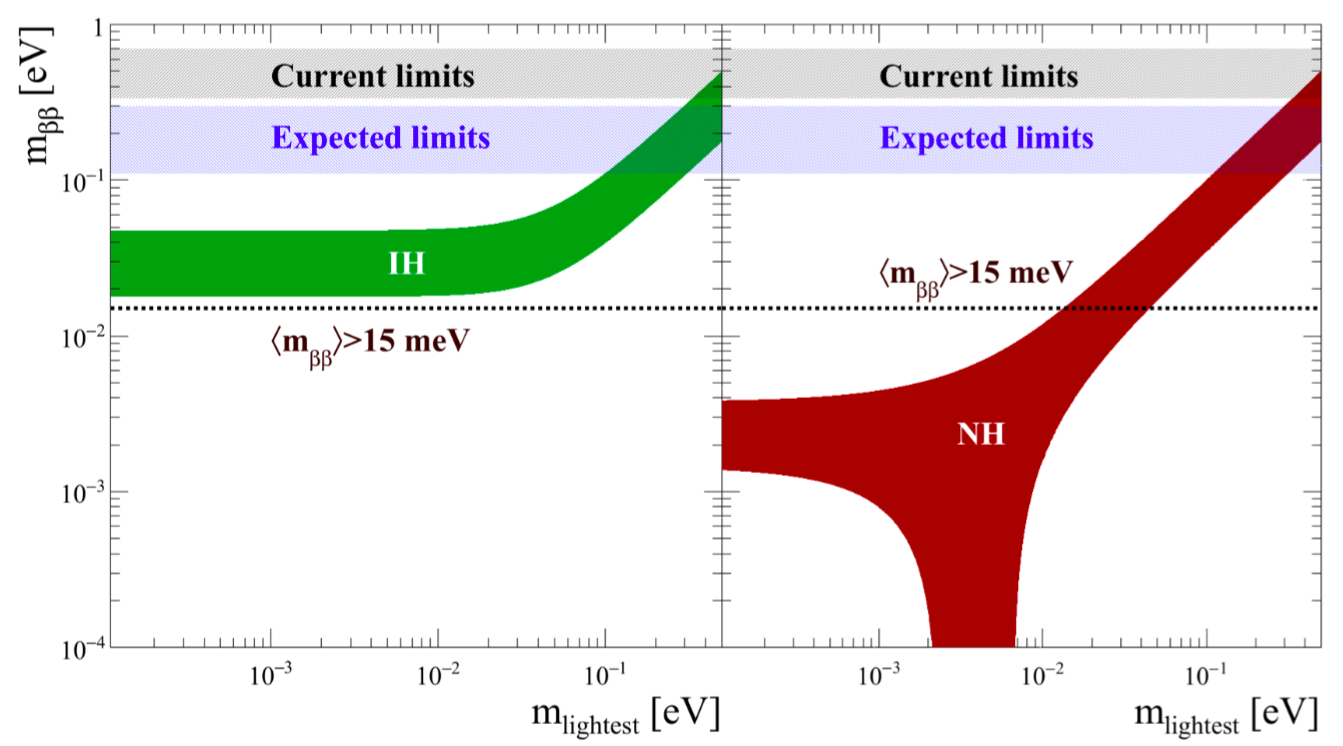
\includegraphics[width=1.0\textwidth]{Neutrinos/NLDBD_sensitivity.png}
\caption{Plot of effective neutrino mass versus the mass of the lightest neutrino in the scenario where NLDBD is mediated by light neutrino exchange. Left corresponds to the inverted hierarchy (green band) and right corresponds to the normal hierarchy (red band). Current limits and expected sensitivities from current generation NLDBD experiments are shown by gray and blue bands. Next generation ``ton-scale'' NLDBD searches will have sensitivities down to $m_{\beta\beta}>15$~meV (dashed line). Figure from~\cite{NSAC}}
\label{fig:NLDBD}
\end{figure}

The complementarity between cosmological neutrino mass measurement and NLDBD can be understood by considering scenarios where NLDBD experiments either observe or fail to observe NLDBD. In the absence of a signal in next generation NLDBD searches, a cosmological measurement constraining $\sum_i m_{\nu i} > 100$~meV (corresponding to either the inverted hierarchy or a minimum neutrino mass of 50~meV) would strongly point to neutrinos being primarily Dirac particles (see Fig.~\ref{fig:NLDBD}). On the other hand, if NLDBD is observed, equation~\ref{eq:mbb} shows that cosmological measurements of $\sum_i m_{\nu i}$ are sensitive to the physics governing neutrino mass generation. For example, Fig.~\ref{fig:MajoranaPhase} shows that in the inverted mass hierarchy cosmological measurements together with NLDBD measurements can constrain one of the Majorana phases. Perhaps even more interesting would be the situation where cosmological and NLDBD measurements violate equation~\ref{eq:mbb} indicating new physics beyond the simple model of light Majorana neutrino mediated decay.

\begin{figure}[h!]
\centering 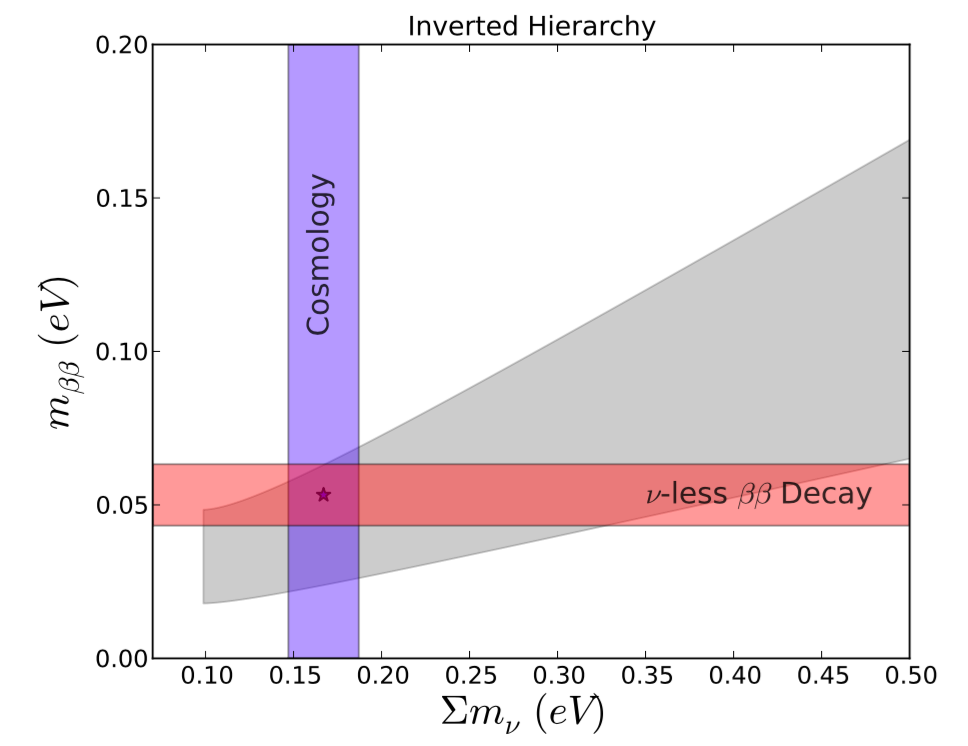
\includegraphics[width=0.70\textwidth]{Neutrinos/IH_MajoranaPhase.png}
\caption{Relationship between effective neutrino mass as measured by NLDBD experiments versus $\sum_i m_{\nu i}$ as measured by cosmology for the inverted hierarchy. The gray band corresponds to a region allowed by existing measurements where the width of the band is determined by the unknown Majorana phase. }
\label{fig:MajoranaPhase}
\end{figure}


%In addition to the effort to constraint the sum of the neutrino masses from cosmology, a variety of lab-based experiments are constraining the angles, phases and masses describing neutrino mixing.  While cosmology is insensitive to mixing angles, 

Cosmological measurements of the summed neutrino masses also complement direct measurements of the neutrino mass using radioactive decay. These kinematic measurements of neutrino mass focus on one of two processes, beta-decay or electron-capture, where the decay spectra near the decay endpoint is particularly sensitive to the mass of the lightest neutrino (add Figure of b-decay and e-capture endpoint spectra).
%to measure the kinematic impact measurements from tritium decay~\cite{Drexlin:2013lha} and neutrino-less double beta decay~\cite{}.

Current kinematic measurements from Mainz~\cite{Kraus:2004zw} and Troitsk~\cite{Aseev:2011dq} limit the neutrino mass to $< 2.0$~eV. The KATRIN experiment~\cite{Angrik:2005ep} will begin taking data in 2016 and is expected to improve this limit by a factor of ten. The spectroscopic techniques of KATRIN are unlikely to improve beyond the $0.2$~eV limit because of the final state spectrum of the source itself, specifically rotational-vibrational states of molecular Tritium. As such, the community is in the process of developing new approaches to kinematic measurements of the neutrino mass. One of the new approaches is a calorimetric measurement of the electron-capture spectrum of $^{163}$Ho. The calorimetric measurement of the $^{163}$Ho endpoint is insensitive to the details of the source configuration and may provide an avenue for eventually surpassing the KATRIN sensitivity. Interestingly, upcoming experiments such as ECHO~\cite{Eliseev:2015pda}, HOLMES \cite{Ceriale:2015mtn}, and NuMECS utilize multiplexed superconducting detectors, the same technology baselined for the CMB-S4 experiment. Another promising direction for direct neutrino mass measurement is the frequency-based technique employed by the Project-8 experiment~\cite{Asner:2014cwa}. Project-8 aims to measure the beta-decay spectrum of Tritium by measuring the frequency of cyclotron radiation emitted by the decay electrons when trapped in a magnetic field. An exciting aspect to this frequency-based technique is the potential to trap atomic Tritium which is not subject to the rotational-vibrational excitations of molecular Tritium. A spectroscopic measurement using atomic Tritium could eventually achieve sensitivities of $<0.04$~eV, a level comparable to cosmological measurements.

%Direct mass measurement from tritium decay works on the following premise.  The $\beta$-decay for tritium produces Helium-3 and an electron and anti-neutrino that carry 18.6 keV of energy between them.  While in most decays this energy is distributed evenly neutrino and electron, there are rare decays where most of the energy is carried by the electron.  If the lightest neutrino is massless, the electron energy may be arbitrarily close to 18.6 eV.  However, for a non-zero mass for the lightest neutrino there is necessary a gap in the electron energy spectrum.  A careful measurement of the electron energy spectrum can therefore constrain the mass of the lightest neutrino.

The relation between cosmological measurement from CMB-S4, kinematic constraints constraints expected from KATRIN~\cite{Angrik:2005ep}, and upcoming long-baseline oscillation experiments is shown in Fig.~\ref{fig:neutrino-noose}. The three approaches to neutrino mass and mixing are complementary and the combination of their results will either reveal new physics in the neutrino sector or provide a definitive measure of the full neutrino mass spectrum.

%The mass of the lightest neutrino is clearly related to the sum of the masses but the lower bound for the sum does not exist for the lightest neutrino.  In this sense the two approaches are complimentary as they cover different aspects of the neutrino mass hierarchy.

\begin{figure}[h!]
\centering 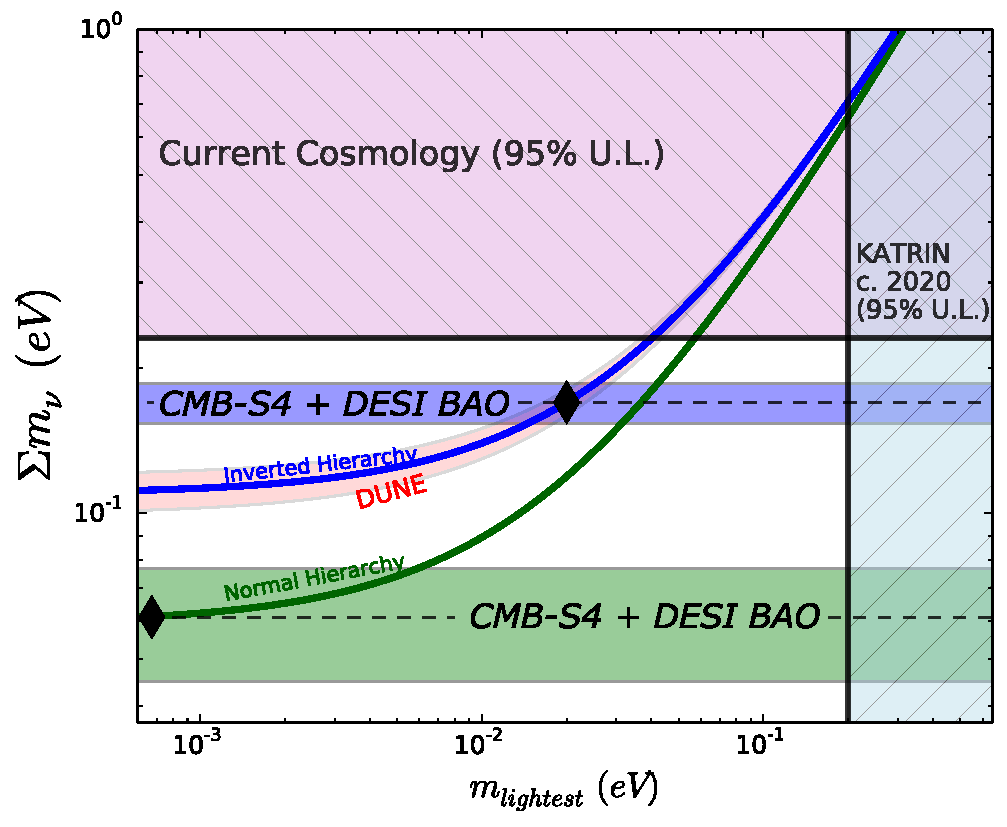
\includegraphics[width=0.55\textwidth]{Neutrinos/numass_combine_dune}
\caption{Shown are the current constraints and forecast sensitivity of
  cosmology to the neutrino mass in relation to the neutrino mass
  hierarchy.  In the case of an ``inverted hierarchy,'' with an
  example case marked as a diamond in the upper curve, the CMB-S4 (with DESI BAO prior)
  cosmological constraints would have a very high-significance
  detection, with $1\sigma$ error shown as a blue band.  In the case
  of a normal neutrino mass hierarchy with an example case marked as
  diamond on the lower curve, CMB-S4 would detect the lowest
  $\sum m_\nu$ at $\gtrsim 3 \sigma$. Also shown is the
  sensitivity from the long baseline neutrino experiment (DUNE) as the
  pink shaded band, which should be sensitive to the neutrino
  hierarchy. Figure adapted from the Snowmass CF5 Neutrino planning document.
 }
\label{fig:neutrino-noose}
\end{figure}

%Neutrinoless double beta decay can occur in a variety of nuclei if neutrinos have a non-zero Majorana mass but does not occur for a Dirac mass.  The decay is effectively involves two neutrons decaying to two protons and two electrons with no associated neutrinos.  The flavor structure of this decay means the amplitude is proportional to $|m_{ee}|^2$ where $m_{ee} = \sum_i m_i U_{ei}$, $U$ is the PMNS matrix, and $m_i$ are the mass eigenstates.  While cosmology can not directly determine whether the mass is Majorana or Dirac, a detection of such a decay could establish that it it has a Majorana mass.  Also, like tritium decay, there is no required lower limit on $m_{ee}$ and therefore there is no level of sensitivity that would guarantee a detection.

Possible anomalies found in short baseline oscillation experiments (LSND~\cite{Aguilar:2001ty},
MiniBooNE~\cite{AguilarArevalo:2010wv}, etc.) may be explained as an active-sterile neutrino
oscillation.  Parameters required to these fits typically lead to
thermalization of the sterile species in the early universe before
neutrino decoupling, resulting in non-standard $N_\mathrm{eff}$ and
contribution to $\sum m_\nu$.  Further description can be found
below in Section~\ref{sec:sterile_neutrinos}.

[AK:6/3] The mass hierarchy may be determined by terrestrial experiments
as well.  NO$\nu$A experiment can determine the hierarchy at
2--3$\sigma$ level if the $CP$-violating phase $\delta_{CP}$ falls into
the favorable range of around $3\pi/2$ ($\pi/2$) for normal (inverted)
hierarchy in a $\sim 5$-year timescale [1].  Possible ambiguity arises
if the nature chooses unfavorable $\delta_{CP}$; this can be resolved by
a future measurement of $\delta_{CP}$ by a next-generation long-baseline
experiment such as Hyper-Kamiokande.  [AK: was there a US competitor of
Hyper-K?  Is it LBNF?]
%
The next-generation US-based long-baseline neutrino-oscillation
experiment, LBNF, is planned to start operation around 2024.
LBNF would resolve the hierarchy at 2--4$\sigma$ level depending on the
$\delta_{CP}$ [2].
%
China-based next-generation reactor neutrino experiment, JUNO, is also
sensitive to the mass hierarchy.  It is scheduled to start data taking
around $\sim$ 2020 and will have $\sim$ 2 (3?)$\sigma$ sensitivity to
resolve the hierarchy after a six-year operation [3].  [AK: I have not
understood what they mean by ``crossing sensitivity.'']
%
Atmospheric neutrino oscillation can also be used to resolve mass
hierarchy [4,5].  KM3NeT/ORCA forecasts to resolve the mass hierarchy at
a 3$\sigma$ level by around 2023.
%
[AK: I have collected schedule information from slides etc., but we may
query PIs of each experiment to get firm citation.]

Cosmological measurements and these terrestrial hierarchy measurements
are complementary to each other.  For example, if cosmology measures the sum of
the neutrino mass heavier than $\sim 116$\,meV, the terrestrial
experiments are the only way to determine the hierarchy.  In turn,
in this case of $\sum m_\nu > 116$\,meV,
determination of the hierarchy by terrestrial experiments would allow
cosmology to constrain the mass of the lightest neutrino without
discrete ambiguity.
In a similar manner to the cosmology being dependent on the central
value of $\sum m_\nu$, 
long-baseline oscillation experiments would suffer from
relatively low sensitivity to the hierarchy
if the $\delta_{CP}$ turns out to be unfavorable.
Also, it is worth noting that all the terrestrial experiments use matter
effect to resolve the hierarchy.  Some of the beyond-the-standard models
involve modification of the neutrino interaction and thus that of the
matter
effect [citation needed].  Cosmological measurements, on the other hand, 
are relatively
insensitive to possible modification of interaction.  Consistency check
between the terrestrial measurements and cosmological constraints would
probe BSM physics in neutrino interaction.

[1] https://doi.org/10.1146/annurev-nucl-102014-021916
[2] https://arxiv.org/abs/1601.05471
[3] https://arxiv.org/abs/1507.05613
[4] http://arxiv.org/abs/1401.2046
[5] http://arxiv.org/abs/1601.07459

\section{Relativistic Species at Recombination}


The angular power spectrum of the cosmic microwave background (CMB) at small angular scales is quite sensitive to the radiation content of the early universe, usually parametrized by a quantity $\Nf$ which will be defined more precisely below.  In the Standard Models of cosmology and particle physics, $\Nf$ is a measure of the energy density of the cosmic neutrino background.  More generally, however, $\Nf$ receives contributions from all forms of radiation apart from photons which are present in the early universe.  Due to its sensitivity to $\Nf$, the CMB can be used as a tool to probe physics of the Standard Model and beyond which are difficult to measure through other means.  Here we will give an overview of the theoretical issues related to $\Nf$ and outline the expectations from the Standard Model.

\subsection{Thermal History of the Early Universe} \label{ThermalHistory}
In this section, we will give a sketch of the thermal history of the standard hot big bang universe when the temperature of the plasma was falling from about $10^{11}$~K to about $10^8$~K following Section 3.1 of \cite{Weinberg:2008zzc}.  For other reviews see \cite{Dolgov:2002wy,Agashe:2014kda}.  During this era, there are two events of particular interest: neutrinos decoupled from the rest of the plasma, and a short time later electrons and positrons annihilated, heating the photons relative to the neutrinos.  Our task is to follow how these events impact the evolution of the energy densities of the photons and neutrinos.

For massless particles described by the Fermi-Dirac or Bose-Einstein distributions, the energy density is given by
\beq
	\rho(T) =
	\Bigg\{\begin{array}{l c l}
        g\frac{\pi^2k_B^4}{30\hbar^3 c^3}T^4 &  &{\rm Boson}\\
       \frac{7}{8}g\frac{\pi^2k_B^4}{30\hbar^3 c^3} T^4 &  &{\rm Fermion}
        \end{array}
\eeq
where $g$ counts the number of distinct spin states.  The entropy density for massless particles is given by
\begin{equation}
	s(T) = \frac{4\rho(T)}{3T} \, .
\end{equation}
It is convenient to define a quantity $\gs$ which counts the spin states for all particles and antiparticles, with an additional factor $\frac{7}{8}$ for fermions.  With this definition, the total energy density and entropy density of the universe during radiation domination are given by
\bea
	\rho(T) &=& \gs\frac{\pi^2k_B^4}{30\hbar^3 c^3}T^4 \, , \nonumber \\
	s(T) &=& \frac{4}{3}\gs\frac{\pi^2k_B^4}{30\hbar^3 c^3}T^3 \, .
\eea
In an expanding universe, the first law of thermodynamics implies that for particles in equilibrium, the comoving entropy density is conserved
\begin{equation}
	a^3s(T) = \mathrm{const} \, .
\end{equation}
One straightforward consequence of this conservation is that for radiation in free expansion, the temperature evolves as the inverse of the scale factor
\begin{equation}
	T\propto \frac{1}{a} \, .
\end{equation}
Let us now apply this to the physics of the early universe.

At a temperature of $10^{11}$~K ($k_BT\sim10$~MeV), the universe was filled with photons, electrons and positrons, and neutrinos and antineutrinos of three species, all in thermal equilibrium with negligible chemical potential, along with a much smaller density of baryons and dark matter both of which are unimportant for the present discussion.  As the temperature of the plasma dropped below about $10^{10}$~K (about 1 second after the end of inflation), the rate of collisions between neutrinos and electrons and positrons could no longer keep up with the expansion rate of the universe, and neutrinos began to fall out of equilibrium and begin a free expansion.  This is just above the temperature for which $m_e c^2 \sim k_B T$, and so for slightly lower temperatures electrons and positrons rapidly disappeared from equilibrium.  We will simplify the discussion by assuming that neutrinos decoupled instantaneously before electron-positron annihilation and comment below how a more detailed calculation modifies the results.  Non-zero neutrino masses can safely be neglected here as long as $m_\nu c^2\lesssim1$~keV which is guaranteed by current observational bounds.

From this point on, we will distinguish the temperature of neutrinos $T_\nu$ from that of the photons $T_\gamma$.  Before neutrino decoupling, frequent interactions kept neutrinos and photons in equilibrium, ensuring they had a common falling temperature.  After the universe became transparent to neutrinos, the neutrinos kept their relativistic Fermi-Dirac distribution with a temperature which fell as the inverse of the scale factor.  The photons, on the other hand, were heated by the annihilation of the electrons and positrons.  Comoving entropy conservation allows us to compute the relative temperatures at later times.

After neutrino decoupling, but before electron positron annihilation, the thermal plasma contained two spin states of photons, plus two spin states each of electrons and positrons, which means that during this period,
\begin{equation}
	g_{\star}^{\mathrm{before}} = 2 + \frac{7}{8}(2+2) = \frac{11}{2} \, .
\end{equation}
After electron positron annihilation, only the two spin states of photons remained, and so
\begin{equation}
	g_\star^{\mathrm{after}} = 2 \, .
\end{equation}
Since $T_\nu\propto a^{-1}$ during this period, we can express the condition of comoving entropy conservation as follows
\begin{equation}
	\frac{g_{\star}^{\mathrm{before}} \, T_{\gamma,\mathrm{before}}^3}{T_{\nu,\mathrm{before}}^3} = \frac{g_\star^{\mathrm{after}} \, T_{\gamma,\mathrm{after}}^3}{T_{\nu,\mathrm{after}}^3} \, .
\end{equation}
Using the fact that $T_{\gamma,\mathrm{before}} = T_{\nu,\mathrm{before}}$, we find as a result
\begin{equation}
	\frac{T_{\gamma,\mathrm{after}}}{T_{\nu,\mathrm{after}}} = \left(\frac{11}{4}\right)^{1/3} \, .
\end{equation}
We find that in the instantaneous neutrino decoupling limit, the annihilation of electrons and positrons raised the temperature of photons relative to that of neutrinos by a factor of $(11/4)^{1/3}\simeq1.401$.

After electron positron annihilation, assuming three species of light neutrinos and antineutrinos, each with one spin state, the radiation density of the universe is
\begin{equation}
	\rho_r = \frac{\pi^2k_B^4}{30\hbar^3 c^3}\left[2T_\gamma^4 + 3\frac{7}{8}T_\nu^4\right] = \frac{\pi^2k_B^4}{15\hbar^3 c^3}\left[1+3\,\frac{7}{8}\left(\frac{4}{11}\right)^{4/3}\right] T_\gamma^4 \, .
\end{equation}
It is conventional to define a quantity $\Nf$ which gives the radiation energy density in terms of the effective number of neutrino species as
\begin{equation}
	\rho_r = \frac{\pi^2k_B^4}{15\hbar^3 c^3}\left[1+\frac{7}{8}\left(\frac{4}{11}\right)^{4/3}\Nf\right] T_\gamma^4 \, .
\end{equation}
In the instantaneous neutrino decoupling approximation described above, we found $\Nf = 3$.  In the real universe, however, decoupling of neutrinos is not instantaneous, and the residual coupling of neutrinos at the time of electron positron annihilation increases $\Nf$ by a small amount in the Standard Model.

The current best estimate of $\Nf$ in the Standard Model is $\Nf = 3.046$ \cite{Mangano:2005cc}.   Unlike photon decoupling at temperature $T \sim 0.2$ eV, active neutrino decoupling at $T \sim 10 \, {\rm MeV} - 0.1 \, {\rm MeV}$ takes place over many tens of Hubble times, with the result that we expect distortions in the relic neutrino energy spectra relative to thermal-shaped, Fermi-Dirac black bodies. Standard Model physics Boltzmann neutrino transport calculations show that these distortions could change $\Neff$ from 3 to something close to 3.05. This result is largely due to (1) the incomplete decoupling of neutrinos during electron-positron annihilation and (2) QED plasma effects.  While both effects have been calculated independently quite accurately, there is some theoretical uncertainty in this quantity due to the various numerical approximations that are made in the calculations when both effects are included simultaneously (see e.g.~\cite{Grohs:2015tfy} for discussion).  








\subsection{Natural Target}

As will be discussed in more detail below, the CMB angular power spectrum is sensitive to the value of $\Nf$ in our universe.  Measurement of the value of $\Nf$ provides a huge amount of insight into the early universe, and is in fact an observational probe of the conditions at very early times, well before recombination.  Even within the Standard Model, $\Nf$ provides an observational handle on the thermal history back to about one second after the end of inflation.  The true power of measuring $\Nf$, however, comes from the realization that it is sensitive not just to the neutrinos of the Standard Model, but it in fact receives contributions from all forms of radiation apart from photons present in the early universe and is thus a probe of new physics.

Collider experiments are known to provide a measurement of the number of neutrino species (or more precisely the number of species of fermions coupling to the $Z$ boson with mass below $m_Z/2$) and find very close agreement with three families of light active neutrinos \cite{ALEPH:2005ab}.  Cosmological measurements of $\Nf$ provide complimentary constraints and are sensitive to the total energy density of radiation whether constituted of active neutrinos or other light species.

If the measured value of $\Nf$ exceeds the Standard Model prediction, it would be an indication that there is additional radiation content in the early universe or that the thermal history is somehow modified.  Additional radiation which contributes to $\Nf$ is often referred to as dark radiation.  There is a large number of possible sources for dark radiation, including sterile neutrinos \cite{Abazajian:2001nj,Strumia:2006db,Boyarsky:2009ix}, gravitational waves \cite{Boyle:2007zx,Stewart:2007fu,Meerburg:2015zua}, dark photons \cite{Ackerman:mha,Kaplan:2011yj,CyrRacine:2012fz}, and many more \cite{Cadamuro:2010cz,Weinberg:2013kea}.  It is also possible that the measured value of $\Nf$ could be found below the Standard Model prediction.  This can happen if for example photons are heated relative to neutrinos after decoupling \cite{Steigman:2013yua,Boehm:2013jpa}.

One of the features that make $\Neff$ a compelling theoretical target is the degree to which broad classes of models fall into two basic levels of $\Delta \Neff$.  As illustrated in Figure~\ref{fig:Neff_thermal}, any species that was in thermal equilibrium with the Standard Model degrees of freedom produces a characteristic correction to $\Neff$ that depends only on its spin and its freeze-out temperature.  For freeze-out after the QCD phase transition, one finds $\Delta \Neff \gtrsim 0.3$.  Freeze-out before the QCD phase transition instead produces $\Delta \Neff > 0.027$.  This first category has been tested by Planck.  The second category, which is sensitive freeze-out temperatures as early as reheating, falls into the level of sensitivity attainable by CMB Stage IV.

\begin{figure}[t!]
\begin{center}
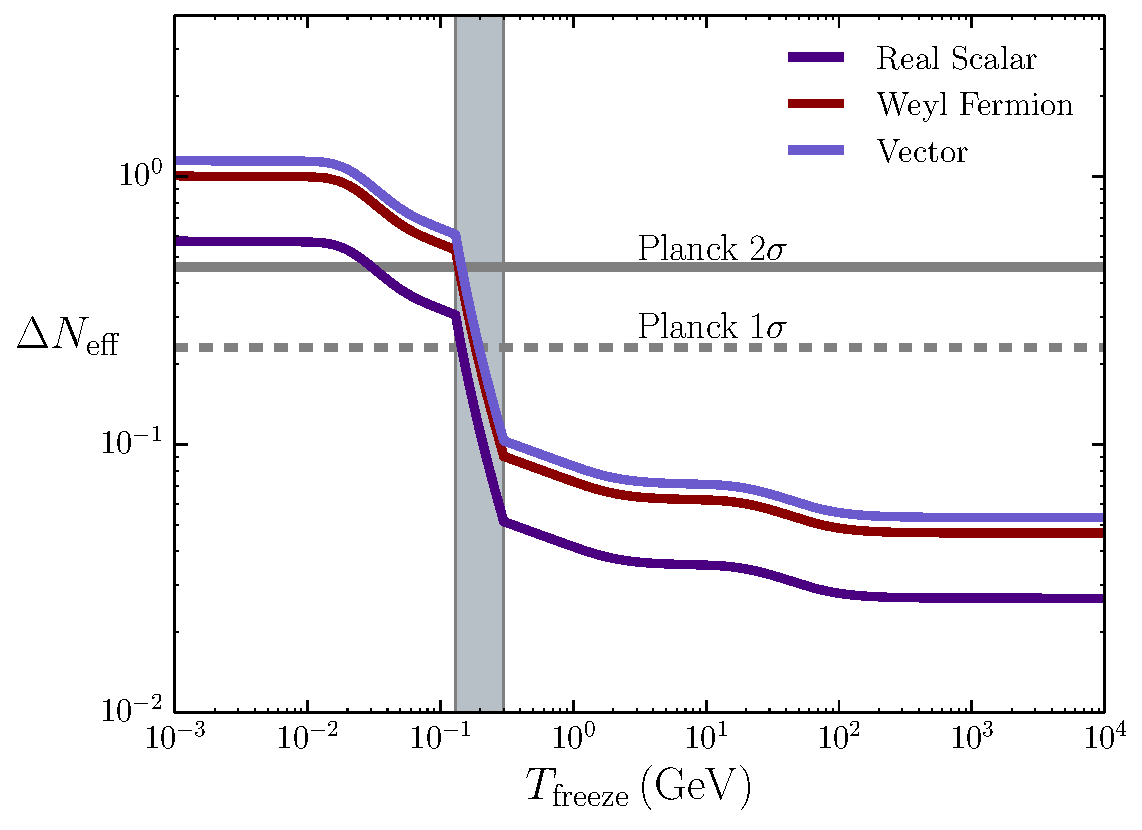
\includegraphics[width=0.65\textwidth]{Neutrinos/Neff.pdf}
\caption{Contribution to $\Neff$ from a massless field that was in thermal equilibrium with the Standard Model at temperatures $T> T_{\rm freeze}$.  For $T_{\rm freeze} \gg m_{\rm top}$, these curves saturate with $\Delta \Neff > 0.027$.   The region in red shows the range of forecasts for $\sigma(\Neff)$ for plausible CMB-S4 configurations. }
\label{fig:Neff_thermal}
\end{center}
\end{figure} 

The contributions to $\Neff$ from hot thermal relics are relatively easy to understand from the discussion of neutrino decoupling.  After freeze-out, the temperature of a relativistic specifics redshift like $a^{-1}$ and therefore is only diluted relative to the Standard Model when energy is injected.  The annihilation of heavy Standard Model particles into photons conserves the comoving entropy and therefore, the diluted temperature of a relic before neutrino decoupling is given by
\beq
%\left( \frac{T_{\rm relic}}{T_{\nu}} \right)^3 = \frac{g_\star (T_{\nu-{\rm freeze-out}})}{g_\star (T_{\rm relic \, freeze-out}) }= \frac{43/4}{g_\star (T_{\rm freeze-out})} *{jm: Changed g* to \mathcal{N} to match notation from above}
\left( \frac{T_{\rm relic}}{T_{\nu}} \right)^3 = \frac{\gs^{\nu-{\rm freeze-out}}}{\gs^{\rm relic \, freeze-out} }= \frac{43/4}{\gs^{\rm relic \, freeze-out}} \, ,
\eeq
where $\gs$ is defined as above to be the number of independent spin states including an additional factor of $\frac{7}{8}$ for fermions.  The order of magnitude difference in $\Delta \Neff$ before and after the QCD phase transition comes from order of magnitude drop in $\gs$ below the QCD scale.  At temperatures well above to top mass, the Standard Model gives $\gs = 106.75$.  

Even a measurement of $\Nf$ which agrees with the Standard Model prediction to high precision would be very interesting due to the constraints it would place on physics beyond the Standard Model.  Some specific implications for sterile neutrinos, axions, and other popular models will be discussed below.  Broadly speaking, constraining $\Delta \Neff$ at the $10^{-2}$ level would constrain or rule out a wide variety of models that are consistent with current cosmological, astrophysical, and lab-based constraints.  Furthermore, because of the sharp change in $\Delta \Neff$ at the QCD phase transition, the improvement from current constraints to projections for CMB Stage IV can be quite dramatic.

For the minimal scenario of a single real scalar, reaching $\sigma(\Neff) \sim 1\times 10^{-2}$ would push the constraint on freeze-out temperatures from electroweak scale to the reheat temperature.  This broad reach to extremely high energies and very early times demonstrates the discovery potential for a precision measurement of $\Nf$ with the CMB.  Furthermore, the CMB power spectrum has the ability to distinguish among certain types of dark radiation based on the behavior of its density perturbations  \cite{Chacko:2015noa,Baumann:2015rya}.  This point will be discussed further below.

A measurement with a slightly larger error on $\Nf$ would still be extraordinarily valuable for higher spin fields, multiple light scalars, and modifications to the thermal history up to the electroweak scale.  In particular, massless fermions and vectors have two helicity states which imply contributions of $\Delta \Neff  \geq 0.047$ and $\Delta \Neff  \geq 0.054$ respectively.  As a result, a less sensitive instrument is still capable of probing physics back to reheating since it could detect or rule out the existence of light thermal relics with non-zero spin.  In addition, there is good reason to think dark sectors could contain multiple light fields which could appear at any level of $\Delta \Neff$ above the minimum contribution from a single scalar field.  Still, the most dramatic jumps in discovery potential occur at the critical values $\Delta \Neff = 0.027, 0.047$, and $0.054$.  

%% Renee Hlozek copied this text from the BSM section - it is currently duplicated %%%

\subsection{Sterile Neutrinos}
\label{sec:sterile_neutrinos}

%\textcolor{red}{(DG:  Needs more basic introduction.  What is a
%  sterile neutrino (include lagrangian) and how does it explain these
%  anomalies?)}

Mechanisms of introducing neutrino mass generally include sterile
neutrinos, with both Majorana and Dirac terms potentially
contributing (e.g., Ref.~\cite{Langacker:2011bi}):
\begin{eqnarray}
\mathcal{L}_D &= -m_D\left(\bar\nu_L\nu_R + \bar\nu_R\nu_L\right)
\mathcal{L}_M &= -\frac{1}{2}m_T\left(\bar\nu_L\nu_L^c + \bar\nu_L^c\nu_L\right) 
-\frac{1}{2}m_S\left(\bar\nu_R\nu_R^c +\bar\nu_R^c\nu_R\right) =
-\frac{1}{2}m_T\left(\bar\nu_a\nu_a\right) -\frac{1}{2}m_S\left(\bar\nu_s\nu_s\right),
\end{eqnarray}
where $\nu_a \equiv \nu_L + (\nu_L)^c$ and $\nu_S \equiv \nu_R +
(\nu_R)^c$ are active and sterile Majorana two component spinors,
respectively. The mass $m_T$ can be generated by a Higgs triplet,
i.e., $m_T = y_T\langle \phi^0_T\rangle$, or from a higher-dimensional
operator involving two Higgs doublets with coefficients
$C/\mathcal{M}$. For dimension 5 operators, this becomes the Type-I
seesaw mechanism, where both Majorana and Dirac terms are present and
$m_S \gg m_D$.


A number of recent neutrino oscillation experiments have reported anomalies
that are possible indications of four or more neutrino mass eigenstates. The
first set of anomalies arose in short baseline oscillation experiments.
First, the Liquid Scintillator Neutirno Detector (LSND) experiment observed
electron antineutrinos in a pure muon antineutrino
beam \cite{Athanassopoulos:1997pv}. The MiniBooNE Experiment also observed
an excess of electron neutrinos and antineutrinos in their muon
neutrino beam \cite{Aguilar-Arevalo:2013pmq}. Two-neutrino oscillation
interpretations of these results indicate mass splittings of $\Delta m^2
\approx 1\rm\ eV^2$ and mixing angles of $\sin^2 2\theta \approx
3\times 10^{-3}$ \cite{Aguilar-Arevalo:2013pmq}. Another anomaly
arose from re-evaluations of reactor antineutrino fluxes that
indicate an increased flux of antineutrinos as well as a lower
neutron lifetime and commensurately increased the antineutrino events
from nuclear reactors by 6\%. This caused previous agreement of
reactor antineutrino experiments to have a $\sim$6\% deficit
\cite{Mention:2011rk,Huber:2011wv}. Another indication consistent with
sterile neutrinos was observed in radio-chemical gallium experiments for solar
neutrinos. In their calibrations, a 5-20\% deficit of the measured
count rate was found when intense sources of electron neutrinos from
electron capture nuclei were placed in proximity to the
detectors. Such a deficit could be produced by a $>1\rm\ eV$ sterile
neutrino with appreciable mixing with electron neutrinos
\cite{Bahcall:1994bq,Giunti:2010zu}. Some simultaneous fits to the
short baseline anomalies and reactor neutrino deficits, commensurate
with short baseline constraints, appear to prefer at least two extra
sterile neutrino states \cite{Conrad:2012qt,Kopp:2013vaa}, but see
Ref.~\cite{Giunti:2015mwa}. Because such neutrinos have relatively
large mixing angles, they would be thermalized in the early universe
with a standard thermal history, and affect primordial nucleosynthesis
\cite{Abazajian:2002bj} and CMB measurements of $\Neff$.

To accomodate $m_S = \mathcal{O}(eV)$ with some mixing between active
and sterile states in the neutrino mass generation mechanism discussed
above requires mixing between active and sterile states with the same
chirality, which does not occur for pure Majorana or Dirac mass cases
or for the conventional seesaw mechanism. One proposed mechanism is
the minimal mini-seesaw ($m_T =0$ and $m_D\ll
m_S\sim\mathcal{O}(\mathrm{eV})$,
e.g. Ref.\cite{deGouvea:2011zz,Donini:2012tt}. In such models, the
sterile neutrinos can have the appropriate masses and mixings to
accommodate the short baseline anomalies. For standard thermal
histories, these sterile neutrinos are typically fully thermalized
\cite{Abazajian:2002bj}. However, it is possible they are partially
thermalized in two extra neutrino models \cite{Jacques:2013xr}.

Interestingly, there are combinations of CMB plus LSS
datasets that are in tension, particularly with a smaller amplitude of
fluctuations at small scale than that inferred in zero neutrino mass
models. This would be alleviated with the
presence of massive neutrinos, extra neutrinos, or both. In particular,
cluster abundance analyses \cite{Wyman:2013lza,Ade:2015fva} and weak lensing analyses
\cite{Battye:2013xqa} indicate a lower amplitude of
fluctuations than zero neutrino mass \cite{Giusarma:2014zza}. Baryon Acoustic
Oscillation measures of expansion history are affected by the presence
of massive neutrinos, and nonzero neutrino mass may be indicated 
\cite{Beutler:2014yhv}, though 2015 Planck results show a lack of such
alleviation in cases with massive or extra neutrinos
\cite{Ade:2015xua}. 

There is a potential emergence of both laboratory and cosmological
indications of massive and, potentially, extra neutrinos. However, the
combined requirements of the specific masses to produce the short
baseline results, along with mixing angles that require thermalized
sterile neutrino states, are inconsistent at this point with
cosmological tension data sets
\cite{Joudaki:2012uk,Archidiacono:2013xxa}. The tension data sets are
not highly significant at this point ($\lesssim 3\sigma$), and there
are a significant set of proposals for short baseline oscillation
experiment follow up \cite{Abazajian:2012ys}. Future high-sensitivity
probes of neutrino mass and number such as CMB-S4 will be able to
definitively test for the presence of extra neutrino number and mass
consistent with sterile neutrinos.

%%%% End of the text copied from BSM section

\subsection{Observational Signatures}

Cosmic neutrinos and other light relics play to two important roles in the CMB that are measured by $\Neff$.  They contribute to the total energy in radiation which controls the expansion history and, indirectly, the damping tail of the power spectrum.  The fluctuations of neutrinos and any other free streaming radiation also produces a constant shift in the of phase the acoustic peaks.  These two effects drive both current and future constraints on $\Neff$.  

The effect of neutrinos on the damping tail drives the constraint on $\Neff$ in the CMB in $\Lambda$CDM + $\Neff$.  The largest effect is from the mean free path of photons, which introduces a suppression $e^{-(k/k_d)^2}$ of short wavelength modes, with~\cite{Zaldarriaga:1995gi}
\beq
k_d^{-2} =\int \frac{da}{a^3 \sigma_T n_e H} \frac{R^2+ \frac{16}{15}(1+R)}{6(1+R)^2} \ ,
\eeq
where $R$ is the ratio of the energy in baryons to photons, $n_e$ is the density of free electrons, and $\sigma_T$ is the Thompson cross-section.  The damping scale is sensitive to the energy density in all radiation through $H \propto \sqrt{\rho_{\rm radiation}}$ during radiation domination (which is applicable at high $\ell$), and is therefore sensitive to $\Neff$ or any form of dark radiation.  From this discussion, we can also see the origin of the degeneracy between $\Neff$ and $n_e$ which may be altered by the primordial helium fraction, $Y_p$.

In reality, the effect on the damping tail is subdominant to the change to the scale of matter radiation equality and the location of the first acoustic peak~\cite{Hou:2011ec}.  As a result, the effect of neutrinos on the damping tail is more accurately represented by holding the first acoustic peak fixed.  This changes the sign of the effect on the damping tail, but the intuition for the origin of the effect (and degeneracy) remains applicable.

In addition to the effect on the Hubble expansion, perturbations in neutrinos affect the photon-baryon fluid through their gravitational influence.  The contributions from neutrinos are well described by a correction to the amplitude and the phase of the acoustic peaks in both temperature and polarization~\cite{Bashinsky:2003tk}.  The phase shift is a particularly compelling signature as it is not degenerate with other cosmological parameters~\cite{Bashinsky:2003tk,Baumann:2015rya}.  This effect is the result of the free-streaming nature of neutrinos that allows propagation speeds of effectively the speed of light (while the neutrinos are relativistic).  Any gravitationally coupled free-streaming light relics will also contribute to the amplitude and phase shift of the acoustic peaks.

E-mode polarization will play an increasingly important role for several reasons.  First of all, the acoustic peaks are sharper in polarization which makes measurements of the peak locations more precise, and therefore aid the measurement of the phase shift.  The second reason is that polarization breaks a number of degeneracies that would also affect the damping tail~\cite{Baumann:2015rya}. \textcolor{blue}{JM: It might be worth mentioning that we can go to higher $\ell_{\rm max}$ with the EE power spectrum, though I guess nobody really knows where foregrounds become a serious issue.}

{\it Status of current observations} -- Planck has provided a strong constraint on $\Neff = 3.15 \pm 0.23$ when combining both temperature and polarization data.  The addition of polarization data has both improved the constraint on $\Neff$ and reduced the impact of the degeneracy with $Y_p$.  Recently, the phase shift from neutrinos has also been established directly in the Planck temperature data~\cite{Follin:2015hya}.  This provides the most direct evidence for presence of free-steaming radiation in the early universe, consistent with the cosmic neutrino background.


\subsection{Forecasts}

\begin{table}[t!]
\begin{center}
\begin{tabular}{l ccc cc} 
 \toprule
    				    			& $1'$  		& $2'$  		& $3'$  		& $\ell_{\rm max} = 3000$	& $\ell_{\rm max} = 4000$ \\ [0.5ex]
 \midrule
   $\sigma(\Neff)$ & -- 		& -- 		& --		& -- 	  	  	& -- 		  \\
    \bottomrule
\end{tabular}
\caption{Forecasts for varying beam size and maximum multipole assuming...}
\label{tab:beam}
\end{center}
\end{table}

% Renee Hlozek cut the text from the BSM section to make a later chapter

\section{Complementarity of CMB and BBN}

%\subsection{Introduction} \label{Introduction}

Primordial light element abundances have historically been an interesting observational test of hot big bang cosmology.  The process by which light elements form in the early universe known as big bang nucleosynthesis (BBN) was worked out theoretically in the early days of the development of the hot big bang model of cosmology \cite{Alpher:1948ve}.  It is a process which depends on all four fundamental forces, that unfolded during the first three minutes of our current phase of expansion, and which has long provided a useful constraint on physics beyond the Standard Model.  The current observational limits on primordial abundances overall show good agreement with the predictions of standard BBN.  Primordial light element abundances are sensitive to the radiation content of the universe as measured through $\Nf$, which also affects the angular power spectrum of the CMB.  Combining these two probes provides useful insight into the physics of the early universe which neither could achieve alone.

\subsection{Standard Big Bang Nucleosynthesis} \label{StandardBBN}
In this section, we will briefly review the physics of big bang nucleosynthesis in the Standard Model.  For more extensive reviews see for example \cite{Weinberg:2008zzc,Agashe:2014kda,Cyburt:2015mya}.

At temperatures above $k_BT\sim 1$~MeV, weak interactions kept neutrons and protons in thermal equilibrium, fixing their number densities to have the ratio $n_n/n_p = e^{-Q/k_BT}$, where $Q = 1.293$~MeV is the mass difference between neutrons and protons.  At lower temperatures, interactions which convert protons to neutrons could not keep up with the expansion rate, leaving free neutron beta decay as the only channel by which protons and neutrons interconverted.  The initial ratio of their number densities at the freeze-out temperature $k_BT_\mathrm{fr}\simeq0.8$~MeV was therefore
\begin{equation}
	n_n/p_n = e^{-Q/k_BT_\mathrm{fr}} \simeq 1/5 \, .
\end{equation}


After freeze-out, neutrons decayed until becoming bound into nuclei.  This process proceeded primarily through two-body processes, starting with the formation of deuterium.  The very small number density of baryons compared to that of photons (parametrized through $\eta\equiv n_b/n_\gamma$) delayed the start of these nuclear reactions until well after the temperature dropped below the binding energy of deuterium due to photo-dissociation of deuterium.  The condition of the onset of deuterium formation is set by requiring that the number of photons per baryon with energy above the binding energy of deuterium drops below unity
\begin{equation}
	\eta^{-1}e^{-|B_D|/k_BT_D} \simeq 1 \, .
\end{equation}
With the deuterium binding energy given by $|B_D|=2.23$~MeV, and $\eta\sim6\times10^{-10}$, we find that deuterium began to form when the temperature dropped below about $k_BT_D\simeq 0.1$~MeV.  By this time, due to free neutron decay, the neutron to proton ratio had dropped to about $n_n/n_p\simeq 1/7$.  Once deuterium was able to form, nearly all of the neutrons quickly became bound into the most energetically favorable light nucleus, which is $\nucl{4}{ }{He}$.  We can estimate the mass fraction of primordial $\nucl{4}{ }{He}$, $Y_p\equiv \frac{\rho\left(\nucl{4}{ }{He}\right)}{\rho_b}$ to be
\begin{equation}
	Y_p = \frac{2(n_n/n_p)}{1+n_n/n_p} \simeq 0.25 \, .
\end{equation}

In addition to $\nucl{4}{ }{He}$, BBN produces a small amount of $\nucl{ }{ }{D}$, $\nucl{3}{ }{He}$, $\nucl{6}{ }{Li}$, and $\nucl{7}{ }{Li}$ (and also $\nucl{7}{ }{Be}$ which subsequently decays by electron capture to $\nucl{7}{ }{Li}$).  While $Y_p$ is primarily sensitive to the neutron lifetime, the primordial abundances of the other light elements depend in complicated ways various nuclear rates and generally require numerical computation (see for example \cite{Wagoner:1966pv,Cyburt:2001pp,Pisanti:2007hk}).

Standard BBN is a one parameter model, depending only on the baryon to photon ratio $\eta$.  The theory predicts several abundances which can be used to fix $\eta$ and check the consistency of the theory, or alternatively, to constrain new physics.  Current observations agree quite well with the predictions of standard BBN, with the exception of $\nucl{7}{ }{Li}$.  It is unclear whether this disagreement points to a problem with the astrophysical determination of the primordial abundance or a problem with the standard theory.  The cosmological lithium problem remains unsolved \cite{Fields:2011zzb}.  From here on, however, we will ignore the lithium problem and focus on how measurements of the other abundances (primarily $\nucl{ }{ }{D}$ and $\nucl{4}{ }{He}$) can be used to constrain the physics of the early universe.




%-----------------------------------------------




\subsection{Beyond the Standard Model}\label{BSM}
Moving beyond standard BBN, measurements of primordial abundances have the ability to constrain many deviations from the standard thermal history and the Standard Model of particle physics.  Because BBN is sensitive to all fundamental forces, changes to any force can in principle impact light element abundances.  Of primary interest for our purpose is that BBN is sensitive to the expansion rate between about one second and a few minutes after the end of inflation.  The expansion rate is in turn determined by the radiation content of the universe during this period, and thus BBN is sensitive to $\Nf$.  

More specifically, the expansion rate determines the freeze-out temperature setting the initial ratio of neutrons to protons and the amount of time free neutrons have to decay.  Additional radiation compared to the Standard Model gives a higher expansion rate, which leads to a higher freeze-out temperature and less time for free neutron decay, leading to a larger primordial $\nucl{4}{ }{He}$ abundance.  The freeze-out temperature also depends weakly on the distribution function of electron neutrinos, though this is subdominant to the dependence $\Nf$ for small non-thermal distortions \cite{Serpico:2004gx}.

Historically, $Y_p$ had provided the best constraint on $\Nf$.  Recent advancements in the determination of primordial deuterium abundance have made constraints on $\Nf$ from deuterium competitive with those from $Y_p$ \cite{Cooke:2013cba}.  The precision with which primordial abundances constrain $\Nf$ is now comparable to that of constraints the CMB power spectrum, and there is no evidence for deviation from the Standard Model \cite{Ade:2015xua}.



%-----------------------------------------------




\subsection{Complementarity with the CMB}\label{Complementarity}
The CMB can be used to quite precisely constrain $\eta$ by measurement of the baryon fraction of the critical density, which is related to $\eta$ by
\begin{equation}
	\Omega_b h^2 \simeq \frac{\eta\times10^{10}}{274} \, .
\end{equation}
Using the value of $\eta$ determined from CMB measurements as an input for BBN makes standard BBN a theory without free parameters which agrees very well with all observations (apart from the aforementioned disagreement with the observed lithium abundance).  The CMB and BBN are sensitive to the baryon density measured at different times.  While BBN is sensitive to the baryon to photon ratio up to a few minutes after the end of inflation, the CMB is sensitive to the baryon density at much later times, closer to recombination about 380,000 years later.  Combining constraints from BBN and CMB on the baryon fraction therefore allows constraints on models where the photon or baryon density changes between these times.

The precision with which the CMB can constrain $\Nf$ will soon come to surpass the constraints from BBN, but the value of the latter will not be totally eclipsed.  BBN and the CMB probe the physics at different times, and so combining constraints can give insight into models where $\Nf$ changes in time.  If it were measured for example that $\Nf^{\mathrm{BBN}}<\Nf^{\mathrm{CMB}}$, this could be explained by the late decay of some unstable particles \cite{Fischler:2010xz,Menestrina:2011mz,Hooper:2011aj}.  Alternatively, if observations revealed that $\Nf^{\mathrm{BBN}}>\Nf^{\mathrm{CMB}}$, this might signal late photon heating \cite{Cadamuro:2010cz,Millea:2015qra}.

The power spectrum of the CMB is also directly sensitive to $Y_p$.  Since helium recombines earlier than hydrogen, the density of helium present at the time of recombination affects the free electron density, and thereby affects the damping tail of the CMB (though in a way which can be distinguished from the effects of $\Nf$) \cite{Bashinsky:2003tk,Hou:2011ec,Follin:2015hya,Baumann:2015rya}.  The degeneracy between $Y_p$ and $\Nf$ is more strongly broken with precise CMB polarization data.

CMB Stage IV will provide constraints on $\Nf$ which are about an order of magnitude better than the current best constraints, and will also improve on the measurement of $Y_p$ by about a factor of two compared to the current best astrophysical measurements.  Combined with measurements of other primordial abundances, this will help to provide a very thorough check of our understanding of the early universe and provide the opportunity to discover physics beyond the Standard Model.

\subsection{Forecasts}


\begin{table}[h!t]
\begin{center}
 \begin{tabular}{l cc} 
 \toprule
   Experiment		& $\sigma(Y_p)$& $\sigma(\Nf)$    \\ [0.5ex] 
 \midrule
   \multirow{2}{*}{Design option 1} 		& -- & --\\
				&-- & --    	     		\\
 \cmidrule{1-3}
   \multirow{2}{*}{Design option 2}			& --  	  & --\\
				& --			& --    	   		\\
 \bottomrule
\end{tabular}
\caption{Forecasts for the marginalized $1\sigma$ errors for $\Neff$ and $Y_p$.    A dash in the $\sigma(\Neff)$ entry indicates that $\Neff = 3.046$ was fixed.  Our forecasts assumed both delensing and lensing reconstruction. }
\label{tab:Yp}
\end{center}
\end{table}





\section{Detection Scenarios for Labs and Cosmology}

The measurement of $\sum m_\nu$ and $\Neff$ from cosmology are complimentary to a wide variety of experiments.  In principle one or more experiment may observe deviations for the standard scenario and the interplay between the different observations will help narrow the space of possibilities. 

\subsection{Neutrino Physics}

As discussed in Section~\ref{sec:lab}, the measurements of the absolute scale of the neutrinos masses from the lab and from cosmology are complimentary in that they are sensitive to different parameters.  In principle, there are a variety of possible scenarios where detections are made both in cosmology and in the lab.  However, given current constraints, most scenarios that involve mostly conventional neutrino physics will result in upper limits from the lab based measurements and a detection of $\sum m_\nu$ and/or $\Delta\Neff \equiv \Neff - 3.046$.  A plausible list of possibilities is shown in Table~\ref{table:neutrinoscenarios}:

\begin{itemize}
\item Conventional neutrino mass scenarios imply majorana masses with a normal or inverted hierarchy.  The normal hierarchy with $\sum m_\nu \simeq 58$~meV is perhaps the most conventional as it reflects the same hierarchical / non-degenerate masses that appear in the charged fermions of the Standard Model.  This scenario is only detectable in the near term via cosmology due to the small size of the neutrino masses.  Somewhat more exotic is the case of a Dirac mass, as it predicts the existence of new light states.

\item The more exotic possibility is that there could be sterile neutrinos that are consistent with a variety of anomalies, as discussed in Section~\ref{sec:sterile_neutrinos}.  In this case, we would observe a correlated signature in both a excess in $\sum m_\nu$ and $\Delta \Neff$.  The sterile neutrino parameters that are most consistent with the anomalies in short-baseline experiments are already in tension with cosmology but would be detected at high significance if true.  

\item Given the current cosmological constraints on $\sum m_\nu$, detections of $m_\beta$ and $m_{\beta \beta}$ in near term experiments would require a significant change to the thermal history.  In particular, a detection of a Majorona mass at the $0.25 \, {\rm eV}$ level would predict a $\sum m_\nu$ that is already excluded by cosmology.  Making the current (or future) limit consistent then requires a mechanism that satisfies both the present bound on $\sum m_\nu$ and the current constraints on $\Neff$.


\item There are a variety of scenarios that produce $\Delta \Neff  \gtrless 0$ without changing neutrino physics.  In this case, the neutrino physics may follow a conventional pattern like the normal hierarchy.  In principle, one would distinguish scenarios where there is no change to the number density of neutrinos (dark radiation) from scenarios where the neutrinos are diluted or enhanced by a change to the thermal history (late decay) as the interpretation of $\sum m_\nu$ depends on the neutrino number density.  However, given that current measurements allow for $< 10$ percent change to the neutrino number density, we would need to detect $\sum m_\nu$ at 10$\sigma$ to be sensitive to such a change.  Nevertheless, dark radiation and changes to the thermal history can make correlated predictions for other experiments as we will discuss in the next subsection.
\end{itemize}
\begin{table}[t!]
\begin{center}
\begin{tabular}
{| l | c c c c | p{5cm} | }\hline Scenario & $m_{\beta \beta}$ & $m_{\beta}$&  $\sum m_\nu$ & $\Delta \Neff$ & Conclusion \\
\hline 
Normal hierarchy & $< 0.15 \, {\rm eV}$ & $< 0.2 \,  {\rm eV}$  & $60 \, {\rm meV}$ & 0 & Normal neutrino physics; no evidence for BSM
\\[.2cm]
Dirac Neutrinos & $< 0.15 \, {\rm eV}$ & $ <0.2 \, {\rm eV}$  & $350  \, {\rm meV}$ & 0 & Neutrino is a dirac particle \\[.2cm]
Sterile Neutrino & $< 0.15 \, {\rm eV}$ & $ <0.2 \, {\rm eV}$   & $350  \, {\rm meV}$ & $>0$ & Detection of sterile neutrino consistent with short-baseline \\
\hline
Bad Cosmology & $ 0.25 \, {\rm eV}$ & $ 0.25 \, {\rm eV}$  & $<150  \, {\rm meV}$ & $0$ & Modified thermal history; (e.g. neutrino decay to new particle) \\[.2cm]
Excluded & $ 0.25 \, {\rm eV}$ & $ 0.25 \, {\rm eV}$  & $500  \, {\rm meV}$ & $0$ & Already excluded by cosmology \\
\hline
Dark Radiation & $< 0.15 \, {\rm eV}$ & $ <0.2 \, {\rm eV}$  & $60  \, {\rm meV}$ & $>0$ & Evidence for new light particles; normal hierarchy for neutrinos
\\[.2cm]
Late Decay & $< 0.15 \, {\rm eV}$ & $ <0.2 \, {\rm eV}$  & $60  \, {\rm meV}$ & $<0$ & Energy-injection into photons at temperature $T \lesssim 1$ MeV \\
\hline 
\end{tabular}
\caption{Relation between neutrino experiments and cosmology.  We include the measurement of the Majorona mass via NLDBD ($m_{\beta \beta}$) or a kinematic endpoint ($m_\beta$) compared to the cosmological measurement of the sum of the masses $\sum m_\nu$ and the CMB measurement of $\Neff$.  For $\Delta\Neff$ the use of $\gtrless 0$ indicates a significant deviation from the Standard Model value.}
\label{table:neutrinoscenarios}
\end{center}
\end{table} 

\subsection{Dark Sectors and Particle Physics}

Deviations from $\Neff = 3.046$ can arise from a wide variety of changes to the particle content and thermal history of the universe.  In most cases, the physics responsible fundamentally requires a coupling of new particles to the Standard Model in regimes where they often can, in principle, be detected by other means.  Cosmology is a very broad tool for searching for beyond the Standard Model physics, but it is also very complimentary to more targeted searches.  A list of plausible detection scenarios is shown in Table~\ref{table:darkscenarios}:
\begin{itemize}
\item Evidence for new massless particles from either experiments or astrophysical observations have immediate implications for cosmology.  Any non-cosmological probe of light particles necessarily requires a coupling of the field to the Standard Model.  A measurement suggesting the strength of the coupling for this particle implies an upper-limit on the freeze-out temperature.  One can then look for the contribution to $\Delta \Neff$ associated with the particle.  If no such contribution is detected, we could place an upper limit on the reheating temperature (or a lower limit for a detection).  Axions present the simplest such examples, as there are a number of experiments that could directly detect axion dark matter (such as ADMX and CASPEr).  A detection in either experiment would predict $\Delta\Neff \geq 0.027$ unless reheating was at sufficiently low temperatures.  The inferred bound in either experiment can be read off of Figures~\ref{fig:axionphoton} or~\ref{fig:axiondipole}.

\item A more complicated example is if a deviation for typical stellar cooling is observed, as has been suggested for white dwarfs.  In this case, there are a number of models that could produce the necessary additional cooling, but would predict $\Delta\Neff \geq 0.027$.  The precise value of $\Delta \Neff$ depends on the spin of the particle and nature of the coupling (which cannot be unambiguously inferred from cooling).  Evidence for additional dark radiation would provide strong support that there is anomalous cooling and would imply a spin for the new light particle through the observed $\Delta \Neff$ using Figure~\ref{fig:Neff_thermal}.

\item Evidence for supersymmetry at the LHC would suggest the existence of a gravitino.  The collider phenomenology of most SUSY models is driven by the precise spectrum of masses of the super partners of the Standard Model fields.  A priori, one may not be able to determine the mass or coupling of the gravitino in a collider.  However, if the gravitino mass is low ($\lesssim$ MeV) then a cosmological abundance of gravitinos is expected.

\item There are a variety of possibilities where we may observe $\Delta \Neff \gtrless 0$ which results from the decay of a massive particle after neutrino decoupling.  A change to $\Neff$ after BBN would imply that $\Neff$ as measured in the CMB could differ significantly from the value inferred from primordial abundances~\cite{Fischler:2010xz}.  From the CMB, we can measure $Y_p$ and $\Neff$ simultaneously which implies such a signature can even be internal to the CMB.  Similarly decays to photons after BBN can also produce $\mu$- or $y$-distortions to the CMB spectrum which could be correlated with $\Delta \Neff < 0$.
\end{itemize}


\begin{table}[t!]
\begin{center}
\begin{tabular}
{| l | c | p{5cm} | p{5cm} | }\hline Scenario & $\Delta \Neff$ & Experimental Input & Conclusion \\
\hline 
Axions & $\geq 0.027$  & Direct detection of axions & lower-limit on the reheat temperature
\\[.2cm]
Low-reheating & $0$  & Direct detection of axions & upper-limit on the reheat temperature
\\[.2cm]    
Stellar Cooling & $\geq 0.027$  & Anomalous Stellar cooling (e.g. white dwarfs) & Evidence for new light particle ; Spin determined by $\Delta \Neff$.  
\\[.2cm]    
Gravitinos & $\geq 0.057$  & LHC evidence for SUSY & upper limit on scale of SUSY breaking
\\[.2cm]  
Late Decays & $< 0$  & Spectral Distortions observed ($\mu$ or $y$) & evidence for new massive particle; energy injection
\\[.2cm]
Evolving $\Neff$ & $> 0$  & Primordial abundances (BBN) consistent with $\Delta \Neff =0$ & Radiation density changed between BBN and Recombination
\\[.2cm]  
\hline 
\end{tabular}
\caption{Relation between particle physics experiments and cosmology.}
\label{table:darkscenarios}
\end{center}
\end{table} 





%%
%% Populate the .bib file with entries from SPIRES Bibtex (preferred)
%% or ADS Bibtex (if no SPIRES entry).
%%  SPIRES will also supply the CITATION line information; please include it.
%%


